% !Tex root=./tb_icml_2018.tex

\section{Convergence of Toy Gaussian Problem}
\label{sec:app:toy-Gauss}

We finish by assessing the effect of the outlined changes in the quality
of the gradient estimates on the final optimization for our toy Gaussian problem.  Figure~\ref{fig:snr/hd_gaussian}
shows the convergence of running Adam~\citep{kingma2014adam} to optimize $\mu$, $A$, 
and $b$.  This suggests that the effects observed predominantly transfer to the overall
optimization problem.  Interestingly, setting $K=1$ and $M=1000$ gave the best performance
on learning not only the inference network parameters, but also the generative network
parameters.
\begin{figure*}[h]
	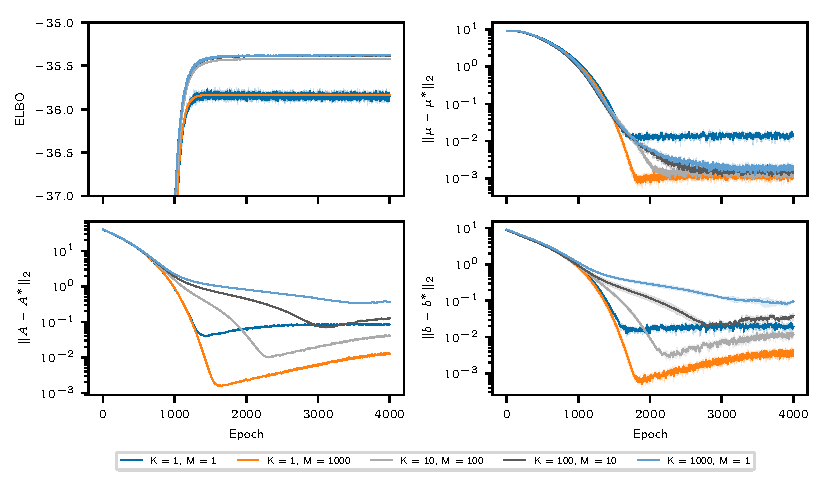
\includegraphics[width=\textwidth]{hd_gaussian.pdf}
	\caption{Convergence of optimization for different values of $K$ and $M$. 
		\emph{(Top, left)} $\ELBO_{\text{IS}}$ during training
		(note this represents a different metric for different $K$). \emph{(Top, right)} $L_2$ distance of the generative network parameters from the true maximizer. \emph{(Bottom)} $L_2$ distance of the inference network parameters from the true maximizer. Plots show means over $3$ repeats with $\pm 1$ standard deviation. Optimization is performed using the Adam algorithm with all parameters initialized by sampling from the uniform distribution on $[1.5, 2.5]$.}
	\label{fig:snr/hd_gaussian}
\end{figure*}